\section{Принцип суперпозиции и интерференция монохроматических волн. Интерференция плоской и сферической волн. Видность полос.}

\theornp{Принцип суперпозиции}{Если в одной точке пространства накладываются колебания двух волн, то они порождают новую волну, равную их векторной сумме.}

Из-за наличия принципа суперпозиции возможно явление интерференции, когда волны взаимно усиляют друг друга, или же наоборот, гасят.

\Def{Монохроматическая волна} --- волна, в спектр которой входит только одна частота.

\subsection{Интерференция двух плоских монохроматических волн. Ширина полосы}

Рассмотрим сперва интерференцию двух плоских монохроматических волн. Пусть распространяются две волны с одинаковой частотой $\omega$:

\begin{align*}
	E_1 &= a_1 e^{i(\vec{k}\cdot \vec{r}_1 - \phi_1)} \cdot e^{-i\omega t}\\
	E_2 &= a_2 e^{i(\vec{k}\cdot \vec{r}_2 - \phi_2)} \cdot e^{-i\omega t}
\end{align*}

Как мы знаем, сами по себе волны складываются. Посмотрим теперь за интенсивностью $I$, которую мы запишем как $I = E E^*$. Распишем суммарную интенсивность (принимаем во внимание, что временная часть в экспоненте одинаковая у всех, поэтому она сократится при произведении с комплексно сопряженным и поэтому следить за ней не будем):

\begin{align*}
	I_{\sum} = (E_1 + E_2) (E_1 + E_2)^* = E_1 E_1^* + E_1 E_2^* + E_2 E_1^* + E_2 E_2^* = \\
	= a_1^2 + 2 a_1 a_2 \cos(k \Delta - \Delta\phi) + a_2^2 = I_1 + I_2 + 2 \sqrt{I_1 I_2} \cos(k \Delta - \Delta\phi)
\end{align*}

Здесь мы ввели $\Delta = r_2 - r_1$, $\Delta\phi = \phi_2 - \phi_1$. Напоминаю, что $k = 2\pi / \lambda$.

\textit{Если же $k_1 \ne k_2$, то вместо $k$ в результирующей формуле будет $K = |k_1 - k_2|$.}

\subsubsection{Ширина полосы}

Рассмотрим чуть более общий случай, когда $|k_1| = |k_2|$, но при этом волны сходятся под некоторым углом $\alpha$. Тогда $K = 2 k \sin(\alpha/2)$

\textbf{Шириной полосы} будем называть расстояние между ближайшими максимумами (\textit{вообще говоря, в МФТИшном конспекте написано что между минимумами, а между максимумами это расстояние между полосами, но наш лектор видимо так не считает, но строго говоря какая разница казалось бы}). В нашем случае она оказывается равной:

\begin{equation*}
	\Delta x = \frac{2\pi}{K} = \frac{2 \pi}{2 k \sin(\alpha/2)} = \frac{\lambda}{2\sin(\alpha/2)} \approx \frac{\lambda}{\alpha}
\end{equation*}

\subsection{Интерференция плоской и сферической монохроматических волн}

Внимание на картинку.

\begin{figure}[H]
	\centering
	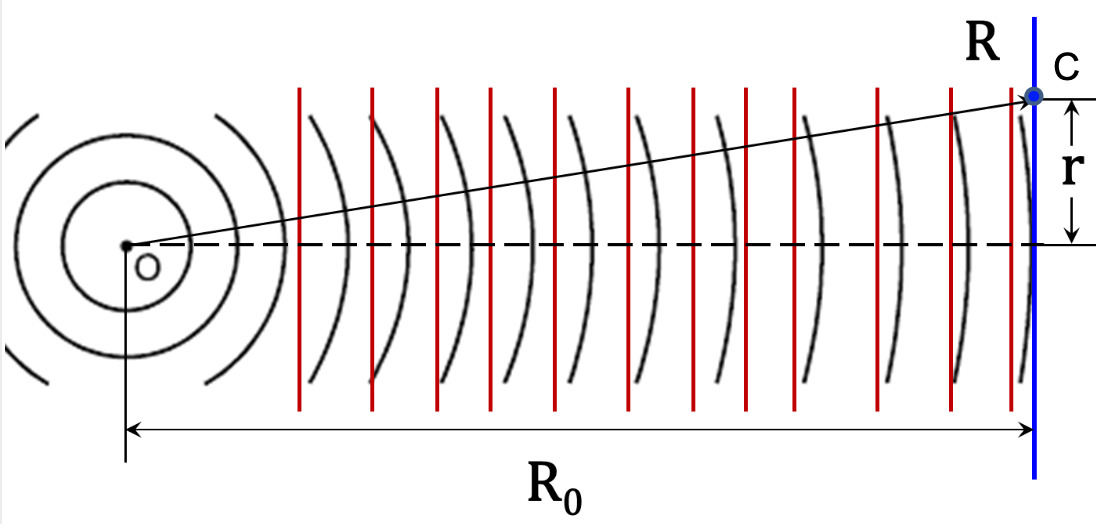
\includegraphics[width=\textwidth]{16_1}
\end{figure}

Будем рассматривать область, где $R_0 \gg r$. При этом:

\begin{equation*}
	R = \sqrt{R_0 + r^2} \approx R_0 + \frac{r^2}{2R_0}
\end{equation*}

Для сферической волны:

\begin{equation*}
	E_{sp} = \frac{a_1}{R_0} e^{i k r} e^{-i \omega t} \approx \frac{a_1}{R_0} e^{i k (R_0 + r^2 / (2 R_0))} e^{-i \omega t}
\end{equation*}

Для плоской волны:

\begin{equation*}
	E_{f} = a_2 e^{i k R_0  - i \omega t}
\end{equation*}

Если это счастье расписать так же, как мы делали с плоской волной, то получим:

\begin{equation*}
	I_{\sum} = \frac{a_1^2}{R_0^2} + a_2^2  + 2 \frac{a_1 a_2}{R_0} \cos \left(k \frac{r^2}{2 R_0}\right)
\end{equation*}

\subsection{Видность}

Для характеристики выраженности интерференции вводят величину, называемую \textbf{видностью} $V$:

\begin{equation}
	V = \frac{I_{max} - I_{min}}{I_{max} + I_{min}}
	\label{eq:Vidnost}
\end{equation}

где $I_{max}$, $I_{min}$ --- максимальное и минимальное значения интенсивности в области интерференции волн.

При интерференции двух \textbf{монохроматических} волн видность будет равна:

\begin{equation*}
	V = \frac{2 \sqrt{I_1 I_2}}{I_1 + I_2}
\end{equation*}